%% arrowLength=10
%% linkWidth=3
%% input fy=50*node.pos
%% output fx=550
%% output fy=50*node.pos+25
%% MAX_FONT_SIZE=8
Imena razredov v glavah matrik zmot so okrašjana zaradi formatiranja dokumenta.
\begin{table}[H]
    \caption{Nabori inicializacijskih parametrov poganjanja na množici Shuttle.}
    \begin{center}
        \begin{tabular}{||l c c c||}
            \hline
            & 1        & 2        & 3 \\ [0.5ex]
            \hline
            velikost populacije               & 200      & 250      & 350      \\
            \hline
            največje število globokih vozlišč & 15       & 20       & 40       \\
            \hline
            največje število povezav          & 30       & 50       & 100      \\
            \hline
            največje število prečkanj         & 2        & 3        & 4        \\
            \hline
            delež mutiranih potomcev          & 10\%     & 10\%     & 10\%     \\
            \hline
            prispevek vozlišč                 & -0.00001 & -0.00001 & -0.00001 \\
            \hline
            prispevek povezav                 & -0.00001 & -0.00001 & -0.00001 \\
            \hline
            število generacij                 & 200      & 250      & 300      \\
            \hline
        \end{tabular}
    \end{center}
    \label{tab:param_statlog}
\end{table}

\subsubsection{Prvi nabor}
%% branch shuttle
%% 200 15 30 2 true 0.1 100 true -0.00001 -0.00001 200 ACC
\begin{table}[H]
    \caption{Rezultat prvega nabora parametrov.}
    \begin{center}
        \begin{tabular}{|| c | c c || c c ||}
            \hline
            \multirow{2}{*}{št. zagona} & \multicolumn{2}{c||}{točnost najboljšega agenta} & \multicolumn{2}{c||}{MCC najboljšega agenta} \\ \cline{2-5}
            & učna    & testna           & učna  & testna         \\
            \hline
            1        & 0\% & 0\% & 0 & 0          \\
            \hline
            2        & 0\% & 0\%          & 0 & 0          \\
            \hline
            3        & 0\% & 0\%          & 0 & 0          \\
            \hline
            4        & 0\% & 0\%          & 0 & 0          \\
            \hline
            5        & 0\% & \textbf{0\%}          & 0 & \textbf{0} \\
            \hline
            $\sigma$ & 0   & 0            & 0 & 0          \\
            \hline
        \end{tabular}
    \end{center}
    \label{tab:statlog_result_1}
\end{table}

\begin{table}[H]
    \centering
    \caption{Matrika zmot najbolj točnega agenta prvega nabora. Agent lahko pravilno napove vse razrede razen \enquote{Fpv Close} in \enquote{Fpv Open}.}
    \begin{tabular}{||rcccccccc||}
        \hline
        razred    & RF    & FC & FO & High & Bypass & BC & BO & vsota \\ \hline
        Rad Flow  & 11398 & 0  & 0  & 76   & 0      & 0  & 4  & 11478 \\ \hline
        Fpv Close & 9     & 0  & 0  & 4    & 0      & 0  & 0  & 13    \\ \hline
        Fpv Open  & 24    & 0  & 0  & 15   & 0      & 0  & 0  & 39    \\ \hline
        High      & 1016  & 0  & 0  & 1139 & 0      & 0  & 0  & 2155  \\ \hline
        Bypass    & 1     & 0  & 0  & 2    & 802    & 4  & 0  & 809   \\ \hline
        Bpv Close & 0     & 0  & 0  & 0    & 0      & 4  & 0  & 4     \\ \hline
        Bpv Open  & 0     & 0  & 0  & 0    & 0      & 0  & 2  & 2     \\ \hline
        vsota     & 12448 & 0  & 0  & 1236 & 802    & 8  & 6  & 14500 \\ \hline
    \end{tabular}
    \label{tab:statlog_acc_1}
\end{table}

%%\begin{table}[H]
%%    \centering
%%    \caption{Matrika zmot agenta z največjim MCC prvega nabora. Agent lahko napove samo razreda \enquote{nesprejemljivo} in \enquote{sprejemljivo}.}
%%    \begin{tabular}{||rccccc||}
%%        \hline
%%        razred       & unacceptable & acceptable & good & very good & vsota \\ \hline
%%        unacceptable & 260          & 103        & 0    & 0         & 363   \\ \hline
%%        acceptable   & 10           & 105        & 0    & 0         & 115   \\ \hline
%%        good         & 0            & 21         & 0    & 0         & 21    \\ \hline
%%        very good    & 0            & 19         & 0    & 0         & 19    \\ \hline
%%        vsota        & 270          & 248        & 0    & 0         & 518   \\ \hline
%%    \end{tabular}
%%    \label{tab:car_mcc_1}
%%\end{table}

\begin{figure}[H]
    \begin{center}
        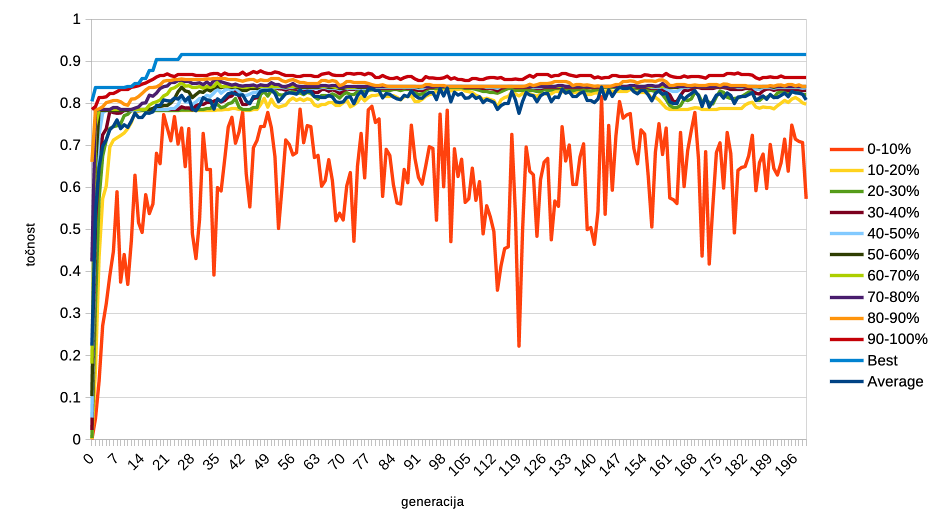
\includegraphics[width=13cm]{statlog/1/acc}
    \end{center}
    \caption{Graf točnosti populacije najboljšega agenta prvega nabora skozi generacije.}
    \label{fig:statlog_acc_1}
\end{figure}

%%\begin{figure}[H]
%%    \begin{center}
%%        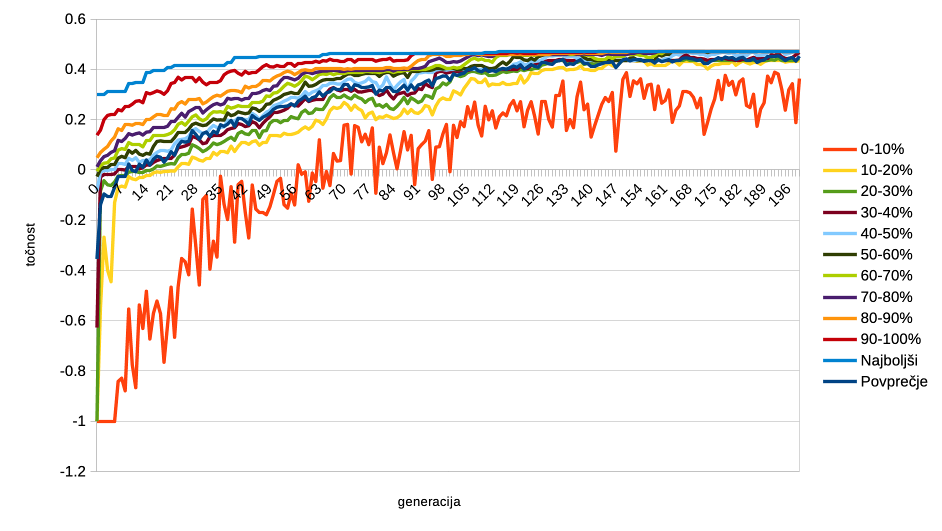
\includegraphics[width=13cm]{car/1/mcc}
%%    \end{center}
%%    \caption{Graf MCC populacije najboljšega agenta prvega nabora skozi generacije.}
%%    \label{fig:car_mcc_1}
%%\end{figure}

\begin{figure}[H]
    \begin{center}
        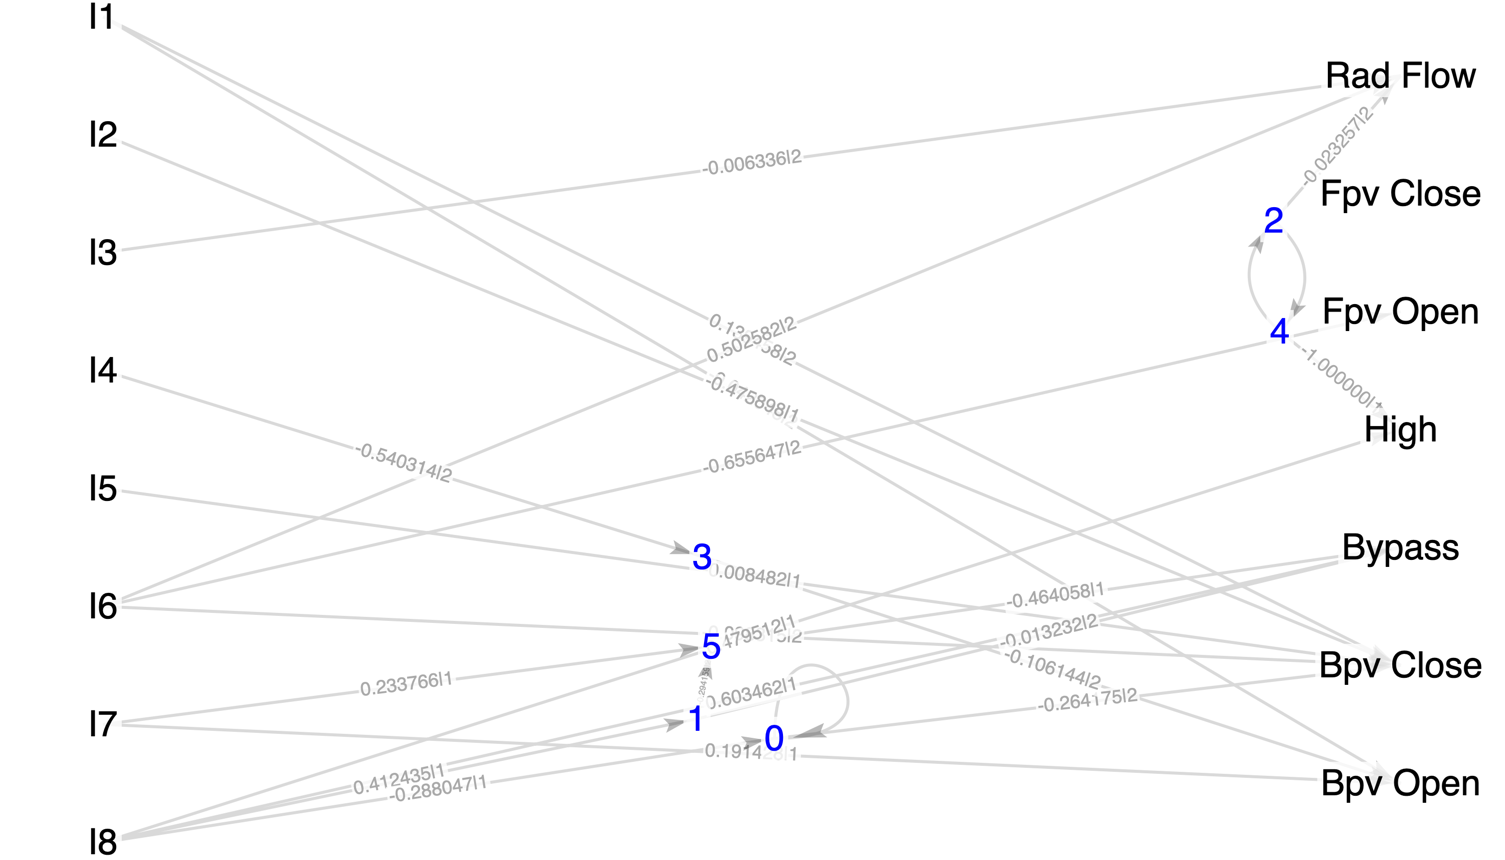
\includegraphics[width=13cm]{statlog/1/acc_g}
    \end{center}
    \caption{Vizualizacija najbolj točnega agenta prvega nabora. Vsebuje 6 globokih vozlišč in 25 povezav.}
    \label{fig:statlog_acc_1_g}
\end{figure}

%%\begin{figure}[H]
%%    \begin{center}
%%        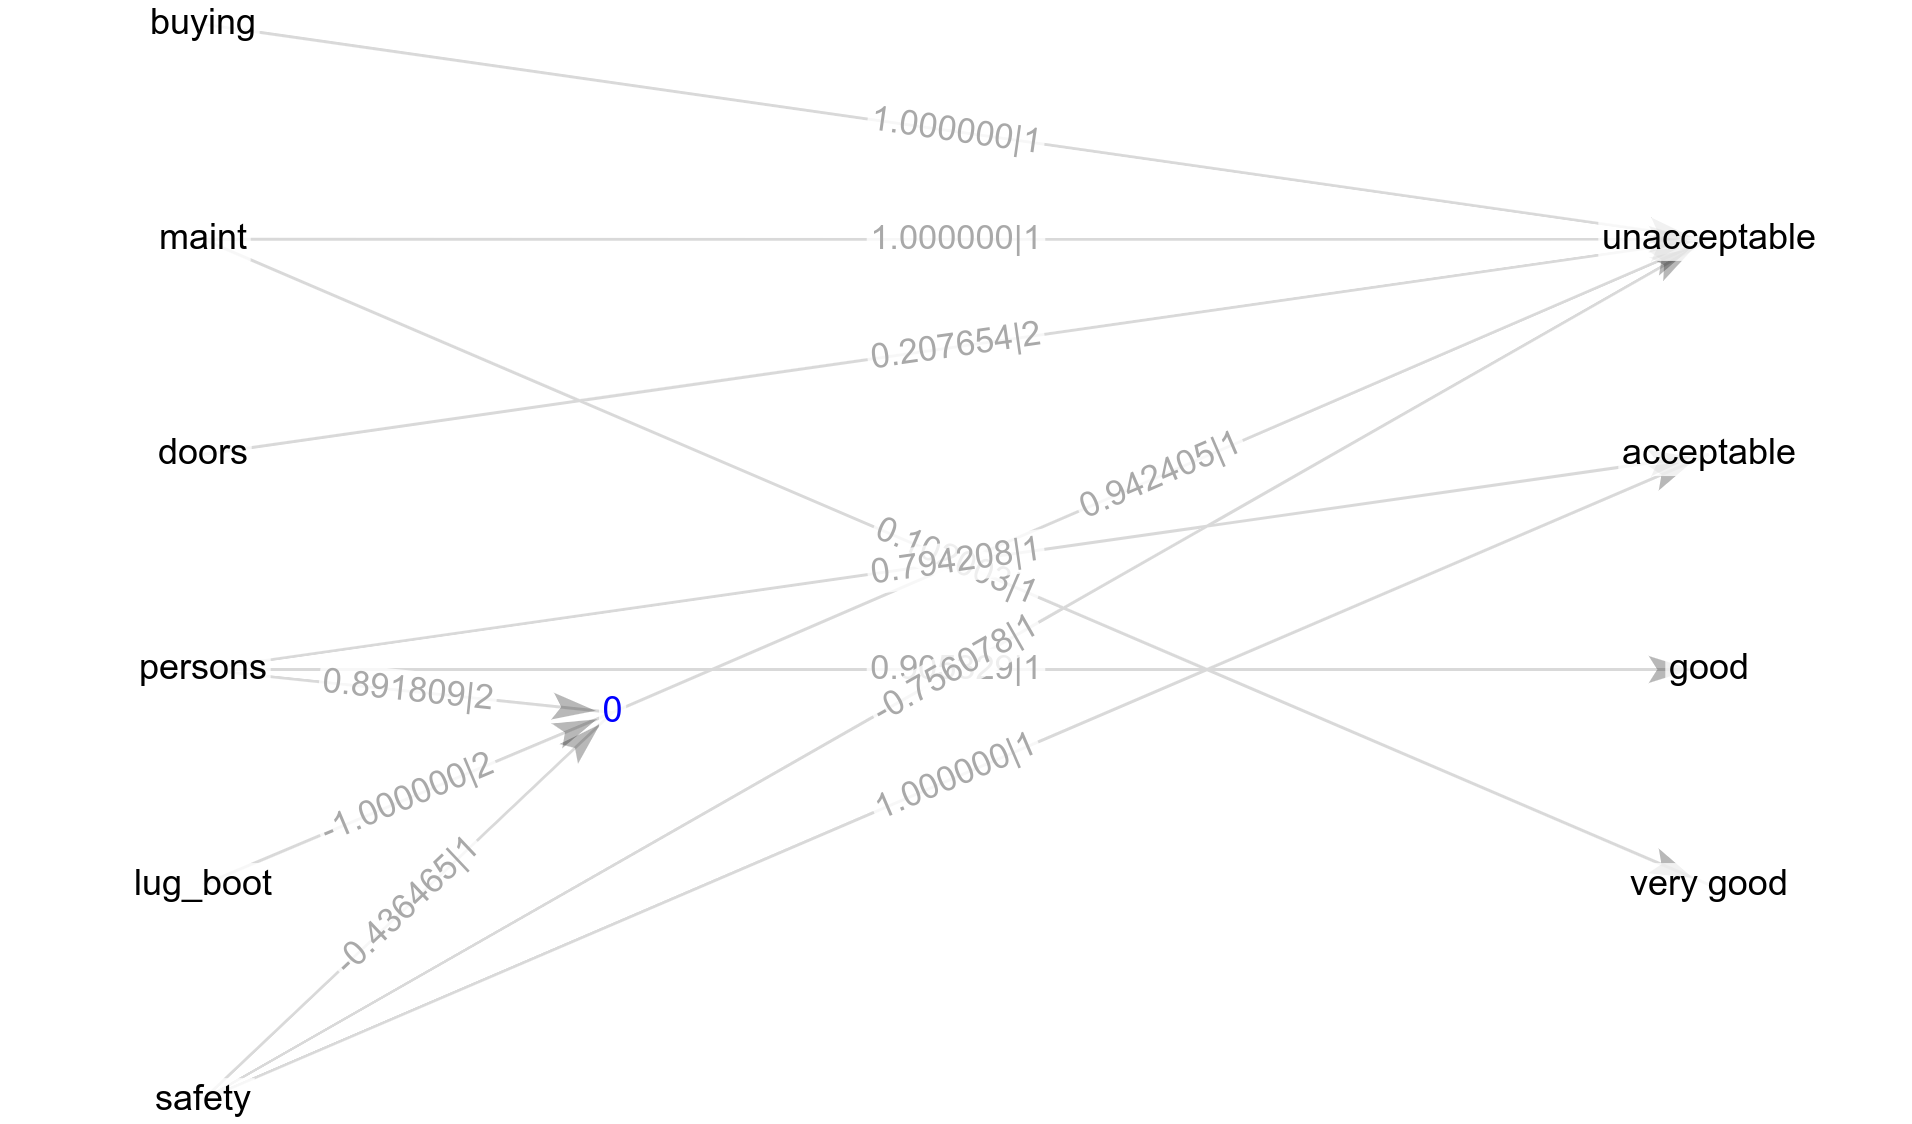
\includegraphics[width=13cm]{car/1/mcc_g}
%%    \end{center}
%%    \caption{Vizualizacija agenta z največjim MCC prvega nabora. Vsebuje 5 globokih vozlišč in 23 povezav.}
%%    \label{fig:car_mcc_1_g}
%%\end{figure}

%\cleardoublepage
%\addcontentsline{toc}{chapter}{Literatura}

%\printbibliography[heading=bibintoc,type=article,title={Članki v revijah}]

%\printbibliography[heading=bibintoc,type=inproceedings,title={Članki v zbornikih}]

%\printbibliography[heading=bibintoc,type=incollection,title={Poglavja v knjigah}]

\printbibliography[heading=bibintoc,title={Celotna literatura}]